\section{Methodology}
\label{sec:methodology}
Fig.~\ref{fig:workflow} presents the experimental workflow for evaluating the effect of slang normalization on Indonesian sentiment classification.

\begin{figure}[t]
\centering
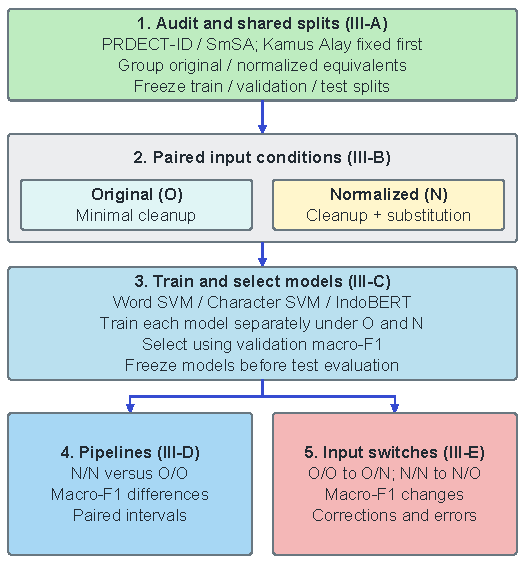
\includegraphics[width=\columnwidth]{figures/proposed_workflow.pdf}
\caption{Workflow for evaluating Indonesian slang normalization. $O$ denotes minimal cleanup and $N$ adds dictionary substitution; each classifier is trained separately on each branch.}
\label{fig:workflow}
\end{figure}

\subsection{Datasets and Partitioning}
PRDECT-ID contains 5,400 Indonesian Tokopedia product reviews across 29 categories, labeled positive or negative~\cite{sutoyo2022}. SmSA contains online comments and reviews with positive, negative, and neutral labels; its released train, validation, and test sets contain 11,000, 1,260, and 500 examples, respectively~\cite{wilie2020}. These are release sizes, not final sample counts. Only review text was used as input; ratings, emotion labels, and product metadata were excluded. SmSA's baseline uses its released, already preprocessed text without additional slang normalization.

The audit checked missing text and invalid labels, then detected duplicates using Unicode NFC normalization, case folding, and whitespace collapsing. Identical canonical texts with agreeing labels retained one representative; conflicting-label groups would be excluded. SmSA duplicates were resolved by partition priority (test, validation, training), then source order; PRDECT-ID used source order. Distinct texts that became identical only after normalization were retained, including any differing labels, because such collisions may reveal information lost through substitution.

Records sharing any canonical original or normalized string formed connected groups within each dataset. PRDECT-ID groups were assigned to approximate 70/15/15 partitions. The deterministic algorithm orders groups by decreasing size, breaks ties using SHA-256 of seed 42 and group identifier, and greedily minimizes squared class-count deficits divided by target counts, plus a total-size term weighted by 0.25. SmSA retained official assignments, with a rule to remove lower-priority members if a group crossed partitions. The dictionary, grouping implementation, tokenizer, and split assignments are jointly fingerprinted. Any change requires a new overlap audit and, if affected, rebuilt splits before training.

The audit removed 112 canonical duplicates from PRDECT-ID and 81 from SmSA's training partition; no missing/invalid records or conflicting-original-label groups were found. Table~\ref{tab:audited-data} gives retained counts; Supplementary Table S4 reports class support by split. SmSA validation and test membership remained unchanged. No canonical original or normalized text crosses partitions. Normalization changes 489 of 793 PRDECT-ID test reviews and 97 of 500 SmSA test reviews; the latter comprise 52 negative, 30 positive, and 15 neutral examples. These subgroup sizes limit the precision of class-specific conclusions.

\begin{table}[t]
\caption{Audited Dataset Partitions}
\label{tab:audited-data}
\centering\small
\renewcommand{\arraystretch}{1.35}
\setlength{\tabcolsep}{5pt}
\setlength{\arrayrulewidth}{0.6pt}
\begin{tabular}{|C{0.25\columnwidth}|C{0.18\columnwidth}|C{0.20\columnwidth}|C{0.18\columnwidth}|}
\hline
\textbf{Dataset} & \textbf{Train} & \textbf{Validation} & \textbf{Test} \\
\hline
PRDECT-ID & 3,702 & 793 & 793 \\
\hline
SmSA & 10,919 & 1,260 & 500 \\
\hline
\end{tabular}
\end{table}

\subsection{Preprocessing and Dictionary Normalization}
Let $O(x)$ denote minimal cleanup: Unicode NFC normalization and trimming and collapsing whitespace. Let $N(x)$ apply dictionary substitution once to $O(x)$. Both conditions retain punctuation, emojis, and negation. Neither includes stemming, stopword removal, edit-distance correction, or other spelling transformations.

The normalizer uses a pinned version of Kamus Alay, associated with the Colloquial Indonesian Lexicon~\cite{salsabila2018}. Dictionary keys and values undergo NFC normalization, case folding, and whitespace cleanup. Eligible keys are single tokens consisting of Unicode letters or decimal digits; replacement values may contain multiple words. Empty replacements and keys with multiple distinct formal alternatives are excluded. Identity mappings do not count as changes. Matching is case-insensitive on complete, maximal letter-or-digit tokens, leaving unmatched text and surrounding symbols unchanged. Replacements use the stored formal value and are not processed again within the same pass.

The pinned dictionary snapshot contains 15,006 rows. Restricting keys to Unicode letters and decimal digits yields 4,202 distinct eligible keys; 71 with conflicting replacements were skipped, leaving 4,131 active mappings. Replacement logs record tokens, replacements, and positions. Four normalized collision groups remain in PRDECT-ID and one in SmSA, none with conflicting labels. Dictionary coverage is an operational measure, not a verified annotation of slang. The policy was checked using constructed examples without manual inspection of test reviews and was fixed before evaluation. On the held-out sets it made 1,527 replacements in PRDECT-ID and 121 in SmSA; counts are operational matches, not verified slang prevalence.

\subsection{Models and Training}
The two datasets, three classifiers, and two preprocessing conditions formed 12 configurations; both conditions used the same retained examples and split assignments. The first two classifiers use word and character TF-IDF with a linear support vector machine (SVM). Word features include unigrams and bigrams over maximal letter-or-digit sequences and individual remaining non-whitespace symbols; character features span three through five characters, including spaces and punctuation. Both analyzers case-fold their inputs. Vocabulary and inverse document frequencies were fitted separately on training data under each condition, with minimum document frequency two, sublinear term frequency, smoothed inverse document frequency, and $L_2$ normalization. Limits were 50,000 word and 100,000 character features.

The contextual classifier fine-tuned the pretrained \texttt{indobenchmark/indobert-base-p1} checkpoint~\cite{wilie2020}, with a linear head on its pooled representation and unweighted cross-entropy updating all layers. A serialized lowercase BERT WordPiece tokenizer uses the pinned vocabulary. Selecting the smallest length in $\{128,256,512\}$ covering at least 95\% of training examples under each condition, including special tokens, yielded 128 for both datasets. Training truncation affects 14 original and 13 normalized PRDECT-ID reviews, and one review per condition in SmSA. All 489 and 97 text-changed test reviews in PRDECT-ID and SmSA, respectively, also produced different word-token sequences and truncated BERT token IDs. A post hoc vector-survival diagnostic found that, among text-changed test reviews, word TF-IDF vectors changed for 488/489 under the original-fitted PRDECT-ID vocabulary and 489/489 under the normalized-fitted vocabulary; vectors changed for 95/97 under either fixed SmSA word vectorizer. Under either fixed character vectorizer, they changed for 489/489 and 97/97, respectively. These counts show any vector change, not the fate of each replacement. A pretrained base checkpoint avoids unknown sentiment-fine-tuning exposure, although pretraining overlap cannot be ruled out.

\begin{table}[t]
\caption{Tuning and Training Settings}
\label{tab:training}
\centering
\small
\renewcommand{\arraystretch}{1.35}
\setlength{\tabcolsep}{5pt}
\setlength{\arrayrulewidth}{0.6pt}
\begin{tabular}{|C{0.27\columnwidth}|C{0.63\columnwidth}|}
\hline
\textbf{Component} & \textbf{Setting} \\
\hline
Linear SVM & $C\in\{0.1,1,10\}$; unweighted classes; squared hinge loss with $L_2$ penalty \\
\hline
IndoBERT search & Learning rate $\in\{2,3,5\}\times10^{-5}$; tuning seed 42 \\
\hline
Optimization & AdamW; weight decay 0.01; effective batch size 16; gradient clipping at 1.0 \\
\hline
Schedule & Five epochs; 10\% linear warmup, followed by linear decay \\
\hline
Selection & Highest validation macro-F1; evaluation after each epoch for IndoBERT \\
\hline
Final runs & SVM: seed 42; IndoBERT: seeds 13, 37, 73 \\
\hline
\end{tabular}
\end{table}

Table~\ref{tab:training} defines equal search budgets across preprocessing conditions: three SVM settings or three transformer tuning runs per model--dataset--condition. SVM training used tolerance $10^{-4}$ and a 20,000-iteration limit; convergence was checked before evaluation. For IndoBERT, bias and layer-normalization parameters were exempt from weight decay, pretrained dropout settings were retained, and batch size was 16. Validation ties favored smaller $C$, or earlier epochs followed by lower learning rates. After learning-rate selection, IndoBERT was retrained from the pretrained checkpoint with three paired seeds, selecting each checkpoint by validation macro-F1. Validation data were not added to training, and the test set did not guide configuration changes. Selected SVM $C$ was 1 except for SmSA word-normalized ($C=10$). Selected IndoBERT learning rates were $2\times10^{-5}$ except for SmSA normalized ($3\times10^{-5}$); Supplementary Table S5 reports final seed-specific epochs. These separately selected settings make the primary difference a full tuning-and-preprocessing pipeline comparison.

\subsection{Evaluation and Uncertainty}
The primary comparison uses separately tuned pipelines; fixed-model diagnostics hold the classifier constant while changing only its evaluation input. Macro-F1 is the primary metric, computed over the fixed label set of each dataset:
\begin{equation}
M=\frac{1}{K}\sum_{k=1}^{K}
\frac{2\mathrm{TP}_k}{2\mathrm{TP}_k+\mathrm{FP}_k+\mathrm{FN}_k},
\end{equation}
where $K$ is two for PRDECT-ID and three for SmSA; a zero denominator contributes zero. Accuracy and per-class performance provide supplementary evidence. For each dataset and classifier, the main effect is
\begin{equation}
\Delta M=M(f_N(N(X)),Y)-M(f_O(O(X)),Y),
\end{equation}
where $f_O$ and $f_N$ are the classifiers trained under the respective conditions, and $(X,Y)$ is the shared test set. Transformer scores and paired differences are summarized by their mean and sample standard deviation across seeds. Absolute scores are not pooled across datasets.

Following the emphasis on effect sizes and uncertainty in NLP evaluation~\cite{bestgen2022}, 95\% percentile bootstrap intervals accompany the differences. We draw 2,000 paired bootstrap samples of test groups with replacement and seed 42. The same samples are used across classifiers, conditions, and transformer seeds; each replicate averages the seed-specific transformer differences. Intervals describe test-sample uncertainty conditional on trained models; seed variability is reported separately.

To test whether normalization benefits the tested word model more than the alternatives, we predefine two contrasts per dataset:
\begin{align}
D_{w,c} &= \Delta M_{\mathrm{word}}-\Delta M_{\mathrm{char}},\\
D_{w,b} &= \Delta M_{\mathrm{word}}-\overline{\Delta M}_{\mathrm{IndoBERT}}.
\end{align}
Each bootstrap replicate recomputes these contrasts on identical sampled reviews. The six pipeline effects and four direct contrasts use nominal intervals, not simultaneous confidence guarantees. A positive effect for one model and an uncertain effect for another does not alone establish a difference between them.

Before classification experiments, we selected 0.01 macro-F1 (one percentage point) as a practical reporting reference. No further rationale was recorded; it is not a community standard. An interval wholly above 0.01 supports a practically meaningful gain within the tested setting; intervals crossing zero or the margin require caution. An interval containing zero does not establish equivalence, and this study is not a powered equivalence test. Per-class harms and introduced errors accompany aggregate interpretation.

\subsection{Input Diagnostics and Error Analysis}
Each selected classifier also predicts both $O(X)$ and $N(X)$, producing the four training/evaluation combinations in Table~\ref{tab:conditions}, without additional training or test-based tuning. For each fixed model, prediction transitions count incorrect-to-correct, correct-to-incorrect, correct-to-correct, and incorrect-to-incorrect cases. This distinguishes input-induced changes from the effects of retraining.

\begin{table}[t]
\caption{Held-Out Macro-F1 for All Training/Input Conditions}
\label{tab:conditions}
\centering\small
\setlength{\tabcolsep}{3pt}
\begin{tabular}{llrrrr}
\hline
\textbf{Data} & \textbf{Model} & $\boldsymbol{O/O}$ & $\boldsymbol{O/N}$ & $\boldsymbol{N/O}$ & $\boldsymbol{N/N}$ \\
\hline
PRDECT & Word & .9570 & .9583 & .9369 & .9646 \\
 & Char. & .9595 & .9646 & .9495 & .9608 \\
 & BERT & .9844 & .9836 & .9810 & .9810 \\
SmSA & Word & .7350 & .7366 & .7358 & .7414 \\
 & Char. & .7214 & .7244 & .7342 & .7317 \\
 & BERT & .8830 & .8836 & .9055 & .9032 \\
\hline
\end{tabular}
\par\vspace{2pt}\raggedright\small First symbol: training condition; second: evaluation input. BERT cells average three paired seeds on the same reviews.
\end{table}

Changed and unchanged reviews are defined by $N(x)\ne O(x)$ before inspecting predictions. Identical inputs must yield identical predictions for a fixed model; this also serves as an implementation check. Any qualitative inspection of corrected and introduced errors is descriptive and does not create new gold labels or estimate linguistic error prevalence. Sentiment improvements alone do not establish semantic preservation.

\subsection{Reproducibility}
The full local workspace retains source checksums, split identifiers, selection records, and per-review predictions. The local snapshot \texttt{review\_snapshot\_v2} includes manuscript and supplement sources, preview PDFs, code, configurations, manifests, and aggregate results; it excludes review-level data and predictions, dictionary mappings, weights, private payloads, and credentials. It is not a public or reviewer-accessible release. The local \texttt{REPRODUCIBILITY.md} guide documents retrieval, auditing, training, inference, analysis, and figure steps; exact replay additionally requires privately retained artifacts, while fresh retraining need not reproduce the same weights. SVM training used Python 3.12.14 and scikit-learn 1.7.1; IndoBERT used Python 3.13.15, PyTorch 2.11.0, Transformers 5.16.1, and one Tesla T4. The cloud image and package inventory were recorded. Resource terms and release status are summarized in the supplement.
